\chapter{Thesis proposal}

% \vspace{-1\baselineskip}
% \setlength\LTleft{-0.5cm}
% \setlength\LTpre{0pt} 
% \setlength\LTpost{0pt}

\begin{longtable}{|p{{{80mm}}}|c|}
\hline
\multicolumn{2}{|m{\linewidth}|}{\textbf{Thesis title}: Deep Fashion with Outfit Recommendation and Try-on}\\
\hline
\multicolumn{2}{|m{\linewidth}|}{\textbf{Advisor}: Dr. Lê Trung Nghĩa - Assoc. Prof. Trần Minh Triết} \\
\hline
\multicolumn{2}{|m{\linewidth}|}{\textbf{Duration}: December 2022 to June 2023}\\
\hline
\multicolumn{2}{|m{\linewidth}|}{
\textbf{Students}: Nguyễn Ngọc Khôi Nguyên (19120106) - Phan Nguyễn Thanh Tùng (19120424)} \\
\hline

\multicolumn{2}{|m{\linewidth}|}{\textbf{Introduction}:\par
The fashion industry is increasingly developing in terms of quantity and quality. Prior to purchasing a garment, customers tend to try them on. However, this fitting process has limitations such as time consumption, the risk of damaging the garments, unavailability of stock, and the need for customers to physically visit the store to try them on.\par

To address this issue, researchers have proposed the "Virtual Try-On" concept to enable customers to see the results of trying on garments without physically going to the store. This idea has opened up various research directions, from 3D technology to augmented reality (AR) and visual feature-based methods.\par

This thesis focuses on the "Visual Feature-based Virtual Try-On" approach. By utilizing deep learning networks, the method takes, as input, an image of a person's pose and combines it with the image of an available garment. The result is an image of the person wearing that particular clothing item. This approach allows customers to easily try on garments anywhere, saving time and enabling them to try out a wider range of clothing options.
}\\
\hline

\multicolumn{2}{|m{\linewidth}|}{\textbf{Objectives}:\par
The research project of the student group focuses on the usability factor while still achieving high effectiveness. Specifically, the input only requires an image of a person and an image of the desired garment to try on. Most existing methods within this category prioritize generating visually appealing try-on images, even if it requires sacrificing processing time. This demands significant hardware capabilities for real-world implementation, thus making widespread application challenging.\par

Therefore, this thesis aims to develop solutions that improve computational speed while maintaining good output quality. The objective is to achieve fast processing while ensuring satisfactory output. These results enable individuals to easily try on garments from fashion stores using a mobile phone or computer, regardless of location. Additionally, this method can pave the way for new avenues of research in visual feature-based virtual try-on.
}\\
\hline

\multicolumn{2}{|m{\linewidth}|}{\textbf{Scope}:\par
The research project focuses on the direction of "Virtual Try-On", with input consisting of an upper-body image of a person and an image of a garment. The output is an image of the person in the input image wearing that particular garment. The objective is to achieve fast processing speed while maintaining comparable try-on results to existing methods.
}\\
\hline

\multicolumn{2}{|m{\linewidth}|}{\textbf{Method}:\par
Research on visual feature-based virtual try-on has attracted significant attention in recent years due to its wide-ranging applications in the fashion industry. Prominent studies such as VITON~\cite{Han-CVPR2018-Viton}, CP-VTON~\cite{Wang-ECCV2018-Toward}, ClothFlow~\cite{Han-ICCV2019-Clothflow}, ACGPN~\cite{Yang-CVPR2020-Towards} work by segmenting the human body into different parts (such as head, hair, arms, upper body, lower body) and/or predicting body joint connections (pose estimation) to enable deep learning models to transform the input garments to fit the body shape appropriately. However, if the segmentation or pose estimation process encounters issues, it can lead to inaccurate virtual try-on results. Moreover, body segmentation algorithms are highly complex, resulting in a significant increase in computational speed.

To address these limitations, recent studies such as như WUTON~\cite{Issenhuth-ECCV2020-Do}, PFAFN~\cite{Ge-CVPR2021-Parser}, Flow-Style-VTON~\cite{He-CVPR2022-Style} have proposed a second approach: utilizing information solely from the person and the clothing images during the virtual try-on image generation process, without the need for segmentation results.

Due to the complex model structure and processing steps involved in the first approach (requiring preprocessing for segmentation and pose estimation), this dissertation primarily adopts the second approach to construct a simpler virtual try-on system. The objective is to provide a solution that balances aesthetic quality and algorithm processing speed, establishing a foundation for practical applications. The proposed solution is expected to utilize a deep learning model, followed by parameter adjustments to achieve the most balanced results in terms of quality and speed.
}\\
\hline

\multicolumn{2}{|m{\linewidth}|}{\textbf{Expected Results}:\par
The expected outcomes of this thesis include the following:\par
\vspace{-4mm}
\begin{itemize}
    \item Experimental results on the accuracy, runtime as well as size of the model.\vspace{-3mm}
    \item The prototype that allows users to generate try-on photos from models and outfits.\vspace{-3mm}
\end{itemize}
}\\
\hline

\multicolumn{2}{|m{\linewidth}|}{\textbf{Research timeline}:\par
\vspace{-4mm}
\begin{itemize}
    \item \textbf{December 2022 - February 2023}: Conduct research for recent methods of using deep learning networks for virtual matching problems.\vspace{-3mm}
    \item \textbf{March - April 2023}: Improved algorithm results on images.\vspace{-3mm}
    \item \textbf{March - April 2023}: Improved algorithm processing speed.\vspace{-3mm}
    \item \textbf{April - May 2023}: Run experiments and compare with recent methods.\vspace{-3mm}
    \item \textbf{June 2023}: Develop an virtual try-on application.\vspace{-3mm}
\end{itemize}
}\\
\hline

\makecell[c]{
\textbf{Advisors} \\
\vspace{2cm}
% \includegraphics[height=2cm]{content/resources/signatures/ltnghia.png}
\\ Dr. Lê Trung Nghĩa \\
% \includegraphics[height=2cm]{content/resources/signatures/tmtriet.png}
\vspace{2cm}
\\ Assoc. Prof. Trần Minh Triết
} 
&
\makecell[c]{
\textbf{Students} \\ 
% 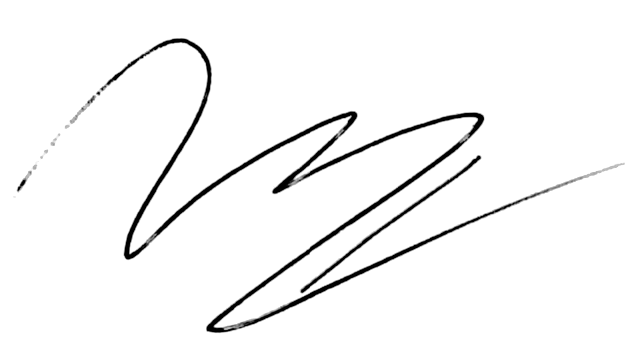
\includegraphics[height=2cm]{content/resources/signatures/nnknguyen.png} 
\vspace{2cm}
\\ Nguyễn Ngọc Khôi Nguyên \\
% 
\includegraphics[height=2cm]{content/resources/signatures/pnttung.png}
\vspace{2cm}
\\ Phan Nguyễn Thanh Tùng 
} \\
\hline
\end{longtable}
